\documentclass[assignment2.tex]{subfiles}
\begin{document}

\section*{2η Άσκηση}
Για την εύρεση της ρίζας της $f(x)=x^3-x-1$ στο διάστημα $Ι=[1,2]$, πρώτα πρέπει να βρεθεί κατάλληλη $g$ τέτοια ώστε $x=g(x) \leftrightarrow f(x)=0$. Πιθανές επιλογές για την $g$ είναι η $g_1(x)=\left(x+1\right)^{\frac{1}{3}}$ και $g_2(x)=x^3-1$. 

``Οπτικά'' η $g_2$ φαίνεται πιο εύκολη επιλογή αλλά $g_2'(x) = 3x^2$ και $g_2'>1$ για $x\in I$, οπότε απορρίπτεται. Επομένως, μένει η $g_1$ η οποία ικανοποιεί το κριτήριο σύγκλισης της ακολουθίας $x_{k+1}=g(x_k)$. Γραφικά, στο Σχήμα \ref{fig:dg2} δίνεται η παράγωγος της $g_1$.
\begin{figure}[hp]
	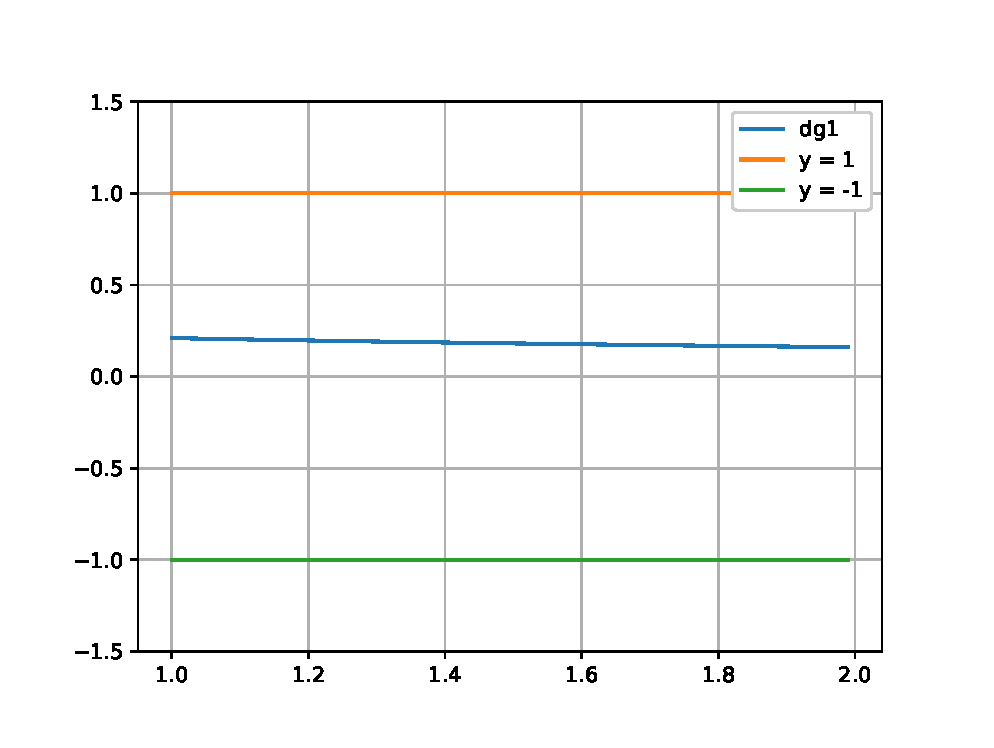
\includegraphics[width=0.7\textwidth]{dg2.eps}
	\centering
	\caption{$g_1'$ στο $I$}
	\label{fig:dg2}
\end{figure} 

Ο αλγόριθμος σταθερού σημείου εκτελείται και συγκλίνει στη ρίζα $\rho=1.32471$ με ακρίβεια $10^{-5}$ όπως ζητείται. Για την επίτευξη της συγκεκριμένης ακρίβειας, απαιτήθηκαν $N=8$ επαναλήψεις. Γραφικά, η ρίζα της εξίσωσης φαίνεται στο Σχήμα \ref{fig:f2}.
\begin{figure}[hp]
	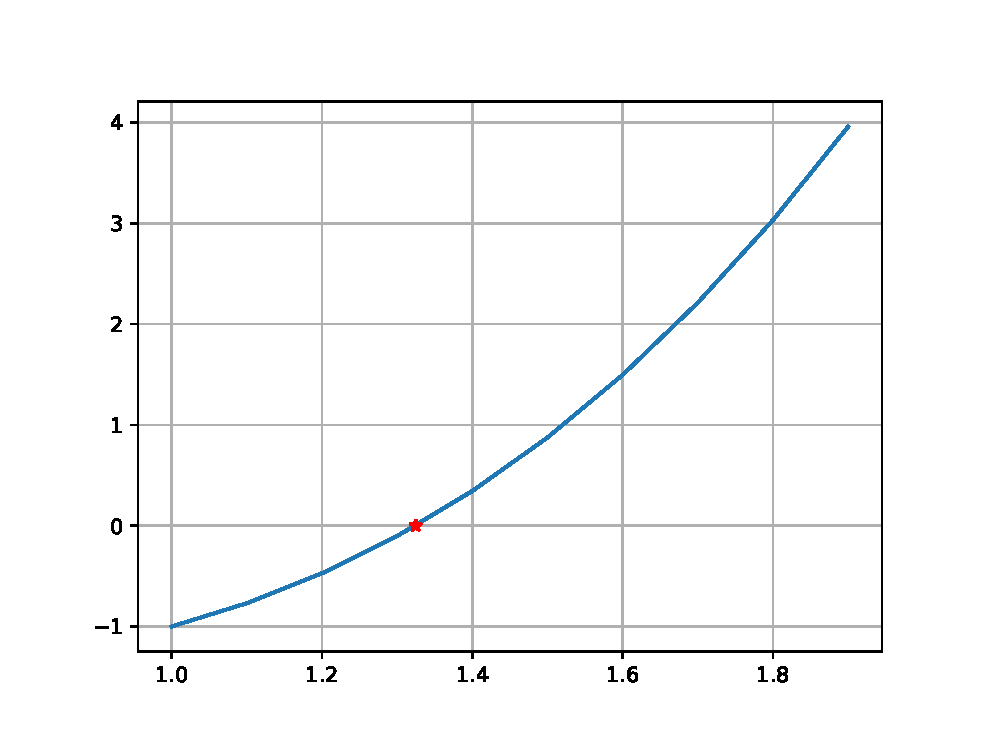
\includegraphics[width=0.7\textwidth]{f2.eps}
	\centering
	\caption{Γράφημα $f(x)=x^3-x-1$ στο $I$}
	\label{fig:f2}
\end{figure}

Παρακάτω ακολουθεί ο κώδικας που γράφτηκε σε \textlatin{Python} και έγινε χρήση της βιβλιοθήκης \textlatin{Numpy}.
\selectlanguage{english}
\lstinputlisting[style=python, firstline=8]{ex2.py}
\end{document}